% Chapter Template

\chapter{Design and Development} % Main chapter title

\label{DesignAndDevelopment} % Change X to a consecutive number; for referencing this chapter elsewhere, use \ref{ChapterX}

\lhead{Chapter \ref{DesignAndDevelopment}. \emph{Design and Development}} % Change X to a consecutive number; this is for the header on each page - perhaps a shortened title

%----------------------------------------------------------------------------------------
%	SECTION 1
%----------------------------------------------------------------------------------------

\section{The design of \theartefact}



%-----------------------------------
%	SUBSECTION 1
%-----------------------------------
\subsection{Requirements}



%-----------------------------------
%	SUBSECTION 2
%-----------------------------------

\subsection{Design}
Common use case:
User comes to site -> Basic site generated from template on server

The user enters URL of page to tag:
	-> URL gets sent to proxy module on server
	-> Proxy fetches the HTML of the target URL
	-> Proxy comments out script and iframe tags
	-> Proxy replaces relative image URIs with absolute image URIs.
	-> Proxy sends back an object containing the sites head and body tag
	-> The content of the body tag is used to populate the content container in the web app.

The user highlights a word on the page to add meta data to:
	-> The text of the highlighted selection gets sent to the lexitags server for disambiguation
	-> The results from lexitags are filtered
		-> If the results contain WordNet terms, then the DBPedia results are filtered away
	-> The results are then sorted
		-> Primarily by source, WordNet terms first, then the first and second level schema.org terms
		-> Secondarily they are sorted lexically
	-> Then the results are displayed on the web page 

	If the user cannot find a match with the highlighted text, 
	it is posible to write your own word into a search box. 
	The semantics of this word will then be linked to the highlighted text.

The user click the sense of the word which match the intended semantics of the highlighted word
	-> The term, either a WN synset or a DBP entity gets sent to the mapping module on the server
	-> The mapping module find the mappings into other ontologies 
		that most closely matches the semantics of the term.
	-> The server returns the entity types that best fit the term, and their namespaces
		-> If no schema.org mapping is found, schema:Thing is returned as it is always correct.
	-> The web app adds a tag which surrounds the selected text, and adds the entity value to it using RDFa
		-> This new tag contains keywords which will highlight it on the page
	-> The web app then asks the server for the schema.org properties of it's schema type(s).
	-> The server returns all the applicable properties
	-> The web app adds all the returned properties to the markup of the page with empty values

The user clicks a marked up section
	-> The web app displays all the possible attributes the section can have
		-> If values have already been inserted, these are shown as the default values
	-> The user inputs the values the attributes should have
	-> When the submit button is click, the attributes get updated to the correct values

The user clicks the export button
	-> The html on the page is cleaned
		-> Temporary markup(tooltips, popover) is removed
		-> Attributes without values are removed
	-> The html is sent to the server
		-> The exporter comments in the script and iframe tags
		-> The html is put in the database
	-> The server returns the id of the new web page
	-> The web app displays the URL to the new marked up website. 

\subsection{Designing the algorithms}
We will now describe the two algorithms that were developed to find mappings between the WordNet synsets and the ontologies.
We use two axes for navigating the WordNet graph, the hypernymes and the hyponymes.
As described in \ref{TheoryWordNet}, a hypernyme can be described as category words into which more specialized words fall.
Hyponyme is the inverse relation, where a hyponyme is a word which can be generalized into some more general category.
For simplicity we will also use one additional term. 
We will use \emph{sibling} to refere to words which are hyponymes of a words hypernyme. 
An example( see figure \ref{Hyponyme}, page \pageref{Hyponyme}) 
would be that \{dog\} has the hypernyme \{domestic\_animal\}, which again have the hyponyme \{cat\},
\{cat\} would then be considered a sibling term of \{dog\}.


Our hopes for this mapping tree is that in the cases where there is no direct mapping from the synset to a term in the 
ontologies we are mapping to, we can always preserve the semantics of the synset by using one of the synsets ancestors.
For the siblings we hope that if we find a mapping, 
then the parent term of the term we have mapped to in the ontology will correspond to the meaning of the synset.
Both these propositions will be tested as a part of the work with the thesis.

The algorithms define different orders of looking at the synsets

\subsubsection{Generating the search tree}
The first step of the algorithm is the same for both algorithms.
A search tree is generated using a perl script 
\footnote{Perl script found at \url{https://raw.github.com/EivindEE/SemTag/master/scripts/parents.pl}.}.

\begin{figure}[h]
    \begin{center}
        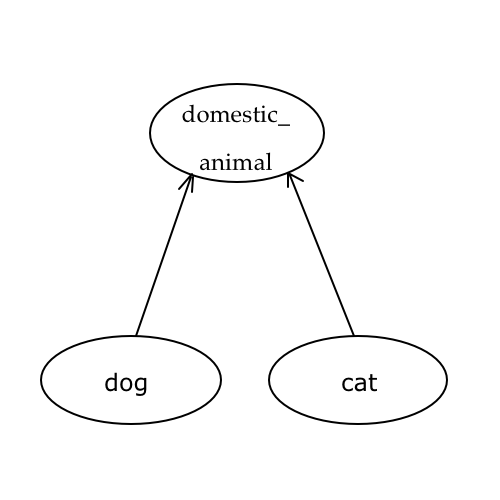
\includegraphics[width=0.60\textwidth]{Hyponyme_own.png}
        \caption{The hyponyme relation, modified from \protect \citet{Miller1990}}
        \label{Hyponyme}
    \end{center}
\end{figure}



\subsubsection{The sibling first algorithm}
The sibling first algorithm traverses the search tree by first looking if there is a direct mapping from the base synset to the ontologies. 
If a direct mapping is not found, it will look at the hypernyms and see if it has a mapping. 
After looking at the hypernyms it will look at the sibling senses. 
It will then go on to look at the hypernyms of the hypernyms, and then their sibling states. 
It will continue to follow the hypernym chain upwards until there are no more hypernyms, or a mappings has been found.

\subsubsection{The ancestors first algorithm}
The ancestor first algorithm will follow the hypernym chain upwards looking for mappings.
The algorithm is written to follow the hypernym chain again, looking at the sibling senses, if no mapping is found.
But since every WordNet noun is a hyponyme of {entity}, which should map to the most general object in an ontology,
it will likely never be touched.
%----------------------------------------------------------------------------------------
%	SECTION 2
%----------------------------------------------------------------------------------------

\section{The ontologies}
Description of the ontologies and why they were chosen

\subsection{Schema.org}

\subsection{Suggested upper merged ontology(SUMO)}

\section{The development process}